%; whizzy chapter
% -initex iniptex -latex platex -format platex -bibtex jbibtex -fmt fmt
% $B0J>e(B whizzytex $B$r;HMQ$9$k>l9g$N@_Dj!#(B

%     Tokyo Debian Meeting resources
%     Copyright (C) 2010 Junichi Uekawa

%     This program is free software; you can redistribute it and/or modify
%     it under the terms of the GNU General Public License as published by
%     the Free Software Foundation; either version 2 of the License, or
%     (at your option) any later version.

%     This program is distributed in the hope that it will be useful,
%     but WITHOUT ANY WARRANTY; without even the implied warranty of
%     MERCHANTABILITY or FITNESS FOR A PARTICULAR PURPOSE.  See the
%     GNU General Public License for more details.

%     You should have received a copy of the GNU General Public License
%     along with this program; if not, write to the Free Software
%     Foundation, Inc., 51 Franklin St, Fifth Floor, Boston, MA  02110-1301 USA

%  preview (shell-command (concat "evince " (replace-regexp-in-string "tex$" "pdf"(buffer-file-name)) "&"))
% $B2hA|%U%!%$%k$r=hM}$9$k$?$a$K$O(Bebb$B$rMxMQ$7$F(Bboundingbox$B$r:n@.!#(B
%(shell-command "cd image201002; ebb *.png")

%%$B$3$3$+$i%X%C%@3+;O!#(B

\documentclass[mingoth,a4paper]{jsarticle}
\usepackage{monthlyreport}
\usepackage{wrapfig}

% $BF|IU$rDj5A$9$k!"Kh7nJQ$o$j$^$9!#(B
\newcommand{\debmtgyear}{2010}
\newcommand{\debmtgmonth}{3}
\newcommand{\debmtgdate}{20}
\newcommand{\debmtgnumber}{62}

\begin{document}
\begin{titlepage}
\thispagestyle{empty}

% $B%?%$%H%k%Z!<%8(B:$BJT=8I,MW$JItJ,$O:G=i$N%^%/%m$KHt$P$9$3$H(B

\vspace*{-2cm}
$BBh(B\debmtgnumber{}$B2s(B $BEl5~%(%j%"(B Debian $BJY6/2q;qNA(B\\
\hspace*{-2cm}

\includegraphics[width=210mm]{image201003/debsen.eps}\\
\hfill{}\debmtgyear{}$BG/(B\debmtgmonth{}$B7n(B\debmtgdate{}$BF|(B\\
%\vspace*{-2.4cm}

\rotatebox{10}{\fontsize{32}{32} {\gt $BFC=8(B1: $B%K%e!<%i%k%M%C%H%o!<%/FC=8(B}}

\rotatebox{10}{\fontsize{32}{32} {\gt $BFC=8(B2: man-db$B$K$O$^$C$F$_$?(B} }

\vspace*{-2cm}
\hfill{}
\includegraphics[height=6cm]{image200502/openlogo-nd.eps}
\end{titlepage}

\dancersection{Introduction}{$B>e@n(B $B=c0l(B}

\begin{multicols}{2}
 
 
 $B:#7n$N(BDebian$BJY6/2q$X$h$&$3$=!#$3$l$+$i(BDebian$B$N@$3&$K$"$7$rF'$_F~$l$k$H(B
 $B$$$&J}$b!"$9$G$K$I$C$W$j$H$D$+$C$F$$$k$H$$$&J}$b!"7n$K0l2s(BDebian$B$K$D$$(B
 $B$F8l$j$^$;$s$+!)(B

 Debian$BJY6/2q$NL\E*$O2<5-$G$9!#(B

 \begin{itemize}
 \item \underline{Debian Developer} ($B3+H/<T(B)$B$N0i@.!#(B
 \item $BF|K\8l$G$N!V(B\underline{$B3+H/$K4X$9$k>pJs(B}$B!W$r@0M}$7$F$^$H$a!"%"%C%W%G!<%H$9$k!#(B
 \item \underline{$B>l(B}$B$NDs6!!#(B
 \begin{itemize}
  \item $BIaCJ$P$i$P$i$J>l=j$K$$$k?M!9$,(B face-to-face $B$G=P2q$($k>l$rDs6!(B
	$B$9$k!#(B
  \item Debian $B$N$?$a$K$J$k$3$H$r8l$k>l$rDs6!$9$k!#(B
  \item Debian$B$K$D$$$F8l$k>l$rDs6!$9$k!#(B
 \end{itemize}
 \end{itemize}		

 Debian$B$NJY6/2q$H$$$&$3$H$G5f6KE*$K$O;22C<TA40w$,(BDebian Package$B$r$,$j$,$j(B
 $B$H:n$k%9!<%Q!<%O%C%+!<$K$J$C$?;Q$rLQA[$7$F$$$^$9!#>pJs$N6&M-!&3hMQ$rDL$7(B
 $B$F(B Debian$B$N:#8e$NG=F0E*$JE83+$X$NEZBf$H$7$F!"!V>l!W$H$7$F$N6u4V$rDs6!$9(B
 $B$k$N$,L\E*$G$9!#(B

\end{multicols}

\newpage

\begin{minipage}[b]{0.2\hsize}
 \definecolor{titleback}{gray}{0.9}
 \colorbox{titleback}{\rotatebox{90}{\fontsize{80}{80} {\gt $B%G%S%"%sJY6/2q(B} }}
\end{minipage}
\begin{minipage}[b]{0.8\hsize}
\hrule
\vspace{2mm}
\hrule
\tableofcontents
\vspace{2mm}
\hrule
\end{minipage}

\dancersection{$B;vA02]Bj(B}{$B>e@n(B $B=c0l(B}

$B:#2s$N;vA02]Bj$O0J2<$G$9(B:

\begin{enumerate}
 \item xxxx
\end{enumerate}

$B$3$N2]Bj$KBP$7$FDs=P$$$?$@$$$?FbMF$O0J2<$G$9!#(B

% 
% this is a prework file.


\dancersection{$B:G6a$N(BDebian$B4XO"$N%_!<%F%#%s%0Js9p(B}{$BA0ED9LJ?(B}
\subsection{$BEl5~%(%j%"(BDebian$BJY6/2q(B61$B2sL\Js9p(B}
% (query-replace-regexp "<.*?>" "")
% (query-replace-regexp "^[	 ]\+" "")

$B:#7n$N(BDebian$BJY6/2q$OLZ99DE9b@l$N65<<$H$=$N6a=j$N8xL14[$r$*<Z$j$7$F(B1$BGq(B2$BF|(B
$B$G3+:E$7$^$7$?!#LZ99DEB&$G2q>l$N=`Hw!";22C<T$NJg=8$r$7$F$/$@$5$C$?:d8}$5(B
$B$s!"Bg;^@h@8!"=IGq<jB3$-$rCf?4$K44;v%5%]!<%H$r$7$F$/$@$5$C$?$d$^$M$5$s!"(B
$B%W%l%<%s%?!<$N3'$5$s(B($B$d$^$M$5$s!"F|HfLn$5$s!":d8}$5$s!">e@n$5$s(B)$B!"$=$7$F(B
$B;22C$7$F$$$?$@$$$?3'$5$s$N$*$+$2$G!"L5;v@.8yN"$K=*$($k$3$H$,$G$-$?$H;W$$(B
$B$^$9!#3'MM$"$j$,$H$&$4$6$$$^$7$?!#(B 

$B%;%C%7%g%s$N;~4VG[J,$d=I$H2q>l$H$N0\F0$,K;$7$J$/$J$C$F$7$^$C$?E@$J$I!"%?(B
$B%$%`%9%1%8%e!<%k$KLdBj$,$"$C$?$N$O;d$N;j$i$LE@$,860x$G$9$N$G!"H?>JE@$H$7(B
$B$F<!2s0J9_$K3h$+$7$?$$$H;W$$$^$9!#(B 

$BJY6/2q$G9T$C$?FbMF$K$D$$$F$O!";vA0G[I[;qNA$dH/I=;qNA!";22C<T$N%V%m%0$K$b(B
$B7G:\$5$l$k$H;W$$$^$9$N$G$3$3$G$OFC$K?($l$^$;$s$,!":#2s$NJY6/2q$NI=8~$-$N(B
$B%F!<%^$O!V4X?t7?8@8l!W!V29@t!W$G$7$?$,!"3+:E$7$F$_$F5$$E$$$???$N%F!<%^$O(B
$B!V1o!W$G$7$?!#$d$^$M$5$s$,;vA02]Bj2sEz!"%;%C%7%g%s$G(BDebian$B$r;H$&M}M3$K(B
$B!V1o!W$r5s$2$F$$$^$7$?$,!"$^$5$K!V1o!W$,$-$C$+$1$G3+:E$G$-!":#2s$NJY6/2q(B
$B$r$-$C$+$1$K?7$?$J!V1o!W$,=PMh$?$J$H;W$$$^$9!#(BDebian$BJY6/2q$rDL$8$?1o0J30(B
$B$K!"4X?t7?8@8l$d%K%e!<%i%k%M%C%H%o!<%/$H$$$C$?6=L#$N$"$kOCBj$rDL$8$?1o!"(B
debian-users$B$N(BML$B$rDL$8$?1o!"(BDebian$B$H(BUbuntu$B$H$$$&%G%#%9%H%j%S%e!<%7%g%s$r(B
$BDL$8$?1o!"0l:rG/$N(BDebian$B29@t$rDL$8$?1o!"$J$I$J$I?'!9$"$j$^$9$,!"FC$K:rG/(B
$B=)$N(BOSC$B$G!VEl5~ET?4$@$1$G$J$/LZ99DE$J$I$N9Y30$G$b3+:E$7$F$[$7$$!W$H:d8}(B
$B$5$s$,MWK>$r=P$7!"8=CO$N44;v$H$7$F<B:]$KF0$$$F$/$@$5$C$?!"$H$$$&$N$,0lHV(B
$BBg$-$J1o$8$c$J$$$+$H;W$$$^$9!#(B 

$B:#=5Kv$K$O(BOSC 2010 Tokyo/Spring$B$,$"$j!"$=$3$GEl5~%(%j%"(BDebian$BJY6/2q$b%V!<(B
$B%9$H%;%C%7%g%s$r=P$9$N$G!":#2s;22C$5$l$?3'$5$s$O$b$A$m$s!";22C=PMh$J$+$C(B
$B$?J}$b!";22C$7$?$3$H$,L5$+$C$?$1$I6=L#$,=P$F$-$?J}$b!"$<$RB-$r1?$s$G$$$?(B
$B$@$1$l$P$H;W$$$^$9!#!V1o!W$r?<$a!"$^$??7$?$J!V1o!W$,$G$-$k$H$h$$$G$9$M!#(B


\dancersection{$B%K%e!<%i%k%M%C%H%o!<%/$G2hA|G'<1$7$F$_$?(B}{$BK\>190E5(B}

\subsection{$B$O$8$a$K(B}

$B%I%-%e%a%s%H%9%-%c%J$GK\$r%9%-%c%s$7$?:]!"2hA|$N%5%$%:$,Bg$-$9$.(B
$B$k$?$aJ]B8$KE,$7$^$;$s!#$3$N2hA|$r#2CM2hA|$H%0%l!<%9%1!<%k!"%+%i!<(B
$B2hA|$=$l$>$l$N=hM}$r2C$($k$3$H$G%U%!%$%k%5%$%:$r=L>.$7!"%K%e!<%i(B
$B%k%M%C%H$rMQ$$$k$3$H$K$h$j$"$kDxEY<+F02=$G$-$J$$$+$H9M$($^$7$?!#(B
$B:#2s$O%K%e!<%i%k%M%C%H$H$7$F0lHLE*$J;0AX%Q!<%;%W%H%m%s$rMQ$$$?2h(B
$BA|H=JL$N0lNc$r2r@b$7$^$9!#(B

\if0
$B%9%-%c%J!<$G2hA|$r%9%-%c%s$9$k$N$K!"%b%N%/%m$H%+%i!<$HJ8;z$N$_$N(B
$B>l9g$o$1$r$9$k$H9bIJ<A$K%9%-%c%s$G$-$k!#(B
$B<jF0$GG'<1$9$k$N$OBgJQ$J$N$G<+F0G'<1$G$-$k$+(B?
\fi

\subsection{$B;0AX%Q!<%;%W%H%m%s$H%P%C%/%W%m%Q%2!<%7%g%s(B}

\subsubsection{$B;0AX%Q!<%;%W%H%m%s(B}

$B;0AX%Q!<%;%W%H%m%s$OF~NOAX!"Cf4VAX!"=PNOAX$HJL$l$?;0AX$N3F%K%e!<(B
$B%m%s$,=E$_$H8F$P$l$k78?t$G7k$P$l$?%b%G%k$H$J$j$^$9!#(B

\begin{figure}[H]
\begin{center}
\caption{$B;0AX%Q!<%;%W%H%m%s(B}
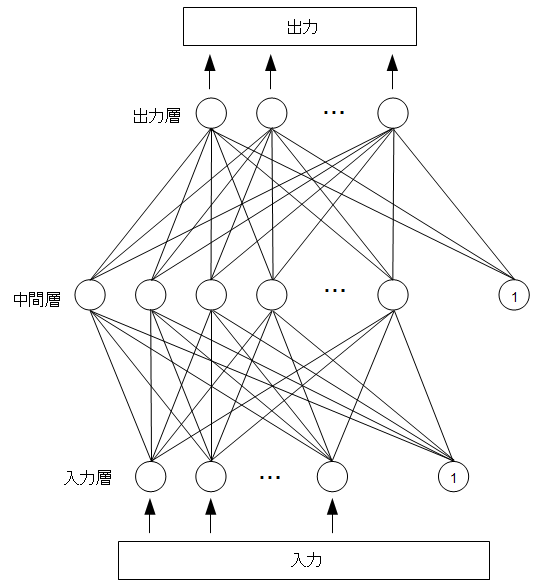
\includegraphics[width=0.45\hsize]{image201003/neuralnet01.png}
\end{center}
\end{figure}

$B$=$l$>$l$N=E$_$O<B?t$GI=$5$l!"%Q!<%;%W%H%m%s$,5!G=$9$k$?$a$K$O$3(B
$B$N=E$_$,E,@Z$K@_Dj$5$l$F$$$kI,MW$,$"$j$^$9!#$"$kF~NO$,M?$($i$l$?(B
$B:]!"F~NOCM$K=E$_$r3]$19g$o$;!"$=$l$>$l$N9g7W$K<!$N$h$&$J%7%0%b%$(B
$B%I4X?t$rE,MQ$7$??tCM$rCf4VAX$N;}$DCM$H$7$^$9!#(B

\begin{multicols}{2}

\begin{figure}[H]
\begin{center}
\caption{$B%7%0%b%$%I4X?t$N<0(B}
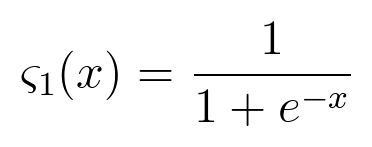
\includegraphics[width=0.5\hsize]{image201003/neuralnet02.png}
\end{center}
\end{figure}

\begin{figure}[H]
\begin{center}
\caption{$B%7%0%b%$%I4X?t$N%0%i%U(B}
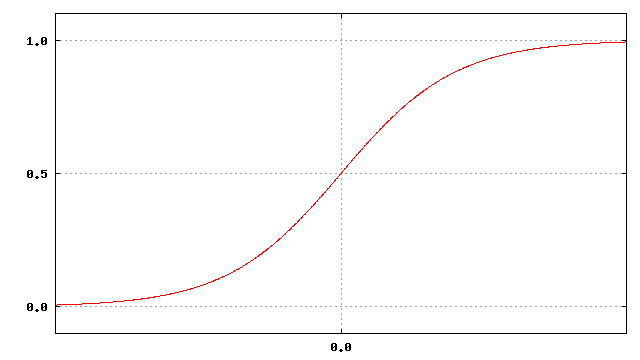
\includegraphics[width=1.0\hsize]{image201003/neuralnet03.png}
\end{center}
\end{figure}

\end{multicols}

$B3F=PNOAX$bF1MM$N7W;;$,$J$5$l!"%Q!<%;%W%H%m%s$N=PNO$,9T$o$l$^$9!#(B

\subsubsection{$B%P%C%/%W%m%Q%2!<%7%g%s(B}

$BB?AX%Q!<%;%W%H%m%s$GE,@Z$J=PNO$r9T$&$?$a$N3X=,J}K!$H$7$F0lHLE*$J(B
$B$b$N$K%P%C%/%W%m%Q%2!<%7%g%s$,$"$j$^$9!#%P%C%/%W%m%Q%2!<%7%g%s$G(B
$B$O$^$:F~NO$KBP$9$k@5$7$$=PNO(B($B65;U?.9f(B)$B$rB??tMQ0U$7!"3F=E$_$r%i%s(B
$B%@%`$K@_Dj$7$^$9!#MQ0U$5$l$?F~NO$KBP$7$F%i%s%@%`$J=E$_$+$i%Q!<%;(B
$B%W%H%m%s$N=PNO$O$G$?$i$a$JCM$H$J$j$^$9$,!"$3$N=PNO$H65;U?.9f$H$N(B
$BHf3S$+$i=PNOAX$HCf4VAX$N4V$N=E$_$r=$@5$7!"<!$$$GCf4VAX$HF~NOAX$N(B
$B=E$_$r=$@5$9$k$3$H$GE,@Z$J=E$_$rC5$7=P$7$^$9!#(B

\subsection{$BB-$7;;$H0z$-;;$r3X=,$7$F$_$k(B}

$B:n@.$7$?%Q!<%;%W%H%m%s$H%P%C%/%W%m%Q%2!<%7%g%s$,@5>o$KF0:n$9$k$+(B
$B$r3N$+$a$^$9!#<!$N$h$&$JF~NO$rMQ0U$7$^$7$?!#(B

\begin{commandline}
# $B3X=,MQ65;U?.9f%Z%"(B
0.40,0.20	0.60,0.20
0.30,0.20	0.50,0.10
0.80,0.10	0.90,0.70
0.20,0.10	0.30,0.10
0.50,0.50	1.00,0.00
0.60,0.20	0.80,0.40
# $BI>2AMQF~NOCM(B
*0.50,0.10
*0.50,0.40
*0.10,0.40
\end{commandline}

$BF~NOCM$H65;U?.9f$N%Z%"$O%?%V6h@Z$j$N:8$,F~NO!"(B
$B1&$,F~NO$KBP$9$k65;U?.9f$G$9!#(B
$B$3$3$G$OB-$7;;$H0z$-;;$N65;U?.9f$rM?$($^$7$?!#(B

\newpage

$B<B9T$7$^$9!#(B

\begin{commandline}
$ ./backprop.exe sample.txt 10000
       0 0.87640153
     100 0.26410368
     200 0.10289131
     300 0.03820243
     400 0.02475167

...($BCfN,(B)...

    9600 0.00077714
    9700 0.00077174
    9800 0.00076646
    9900 0.00076128
0.4000, 0.2000  0.60, 0.18      0.60, 0.20
0.3000, 0.2000  0.50, 0.11      0.50, 0.10
0.8000, 0.1000  0.90, 0.70      0.90, 0.70
0.2000, 0.1000  0.30, 0.11      0.30, 0.10
0.5000, 0.5000  0.98, 0.02      1.00, 0.00
0.6000, 0.2000  0.80, 0.41      0.80, 0.40
0.5000, 0.1000  0.63, 0.35
0.5000, 0.4000  0.93, 0.06
0.1000, 0.4000  0.87, 0.00
Ratio=0.00075626
Count=10000
Sample=6
Input=2
Middle=4
Output=2
InputHidden0=-2.57936471,-2.20525001,-1.50656422,4.05055823,-0.66468037
InputHidden1=-1.29032439,8.71632107,-1.24344376,-0.85214732,-0.66468037
InputHidden2=2.04901840,-2.94096519,1.04866634,-1.98825291,0.29698485
HiddenOutput0=-2.91458436,-1.16992032
HiddenOutput1=5.84673832,-6.31188860
HiddenOutput2=-1.80018561,-0.42470539
HiddenOutput3=3.60356071,3.84028669
HiddenOutput4=1.40998866,-1.22885398
\end{commandline}

$BMj$j$J$$$J$,$i$b$=$l$J$j$N1i;;7k2L$,=PNO$5$l$F$$$^$9!#I>2A$H$7$F(B
$B:G8e$N?tCM$O8:;;7k2L$,Ii$K$J$k$O$:$J$N$G$9$,!"%7%0%b%$%I4X?t$rDL(B
$B$9$3$H$G=PNO$,(B0.0$B!A(B1.0$B$H$J$k$?$a@5>o$J7k2L$,F@$i$l$^$;$s!#(B

\subsection{$B2hA|$rJ,N`$9$k$?$a$NF~NOCM$r9M$($k(B}

$B2hA|H=JL$NF~NOCM$H$7$F<!$NCM$r;HMQ$7$^$7$?!#(B

\begin{itemize}
\item $BJd@5$7$?2hA|$N(BRGB$B$N:9(B
\item $BHyJ,$7$?2hA|$N(BRGB$B$N:9(B
\item $B2hA|$NJ#;($5!#(B
\item $B;H$o$l$F$$$k?'$N?t(B
\item $BJ?6Q:LEY(B
\item FFT$B=hM}$7$?2hA|$NL@$k$$%T%/%;%k$rMxMQ$9$k(B
\item HSV$B$KJQ49$7!"?'AG$NJ?6Q$rMxMQ$9$k(B
\item $B?'AG$NJ,;6$rMxMQ$9$k(B
\end{itemize}

$B$3$NCf$+$iJ8>O$H3($NH=JL$H$7$F2hA|$N(BFFT$B$r!"%+%i!<2hA|$NH=JL$H$7(B
$B$F(BHSV$B$X$NJQ49$r2r@b$7$^$9!#(B

\newpage

\subsubsection{$B%b%N%/%m2hA|$N=hM}!&J8;z$H3($rJ,N`$7$F$_$k(B}

$B=D=q$-$NJ8>O$O2#J}8~$K0lDj$N<~GH?t$r;}$C$F$$$k$H8+$J$9$3$H$,=PMh(B
$B$^$9!#$3$l$K$h$j!"J8>O$N2hA|$rHyJ,$7(BFFT$B=hM}$r9T$C$?7k2L$+$i?6I}(B
$B$rIA2h$9$k$H$G!"L@$k$/8w$kE@$,8=$l$k$3$H$,$o$+$j$^$7$?!#(B

\begin{figure}[H]
\begin{center}
\caption{$B%$%i%9%H$HJ8>O$rHyJ,$7$?2hA|$N(BFFT$B7k2L(B}
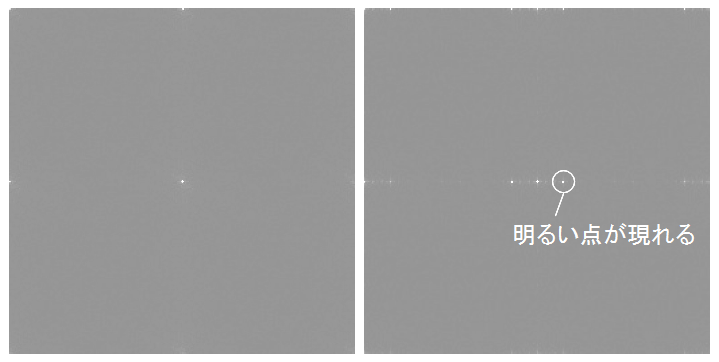
\includegraphics[width=0.9\hsize]{image201003/neuralnet04.png}
\end{center}
\end{figure}

$B$3$NE@$NL@$k$5$rF~NOCM$H$9$k$3$H$G!"J8>O$H%$%i%9%H$NH=JL$,9T$($k(B
$B$H4|BT$G$-$^$9!#(B

\if0
$BFs<!85(BFFT$B$G=hM}$7$?7k2L(B

$BHyJ,$7$FFs<!85(BFFT$B$G=hM}$7$?7k2L(B
\fi

\subsubsection{$B%+%i!<2hA|$H$=$&$G$J$$2hA|$rJ,N`$7$F$_$k(B}

$B%+%i!<2hA|$H%b%N%/%m2hA|$O2hA|$N(BRGB$B$r(BHSV$B$KJQ49$7!"?'Aj$+$iH=JL$r(B
$B9T$C$F$$$^$9!#(B

RGB$B$N$&$A$+$i:GBg$N$b$N$r(BMAX$B!":G>.$N$b$N$r(BMIN$B$H$9$k$H?'Aj$O<!$N(B
$B<0$H$J$j$^$9!#(B

\begin{figure}[H]
\begin{center}
\caption{$B?'Aj$N7W;;<0(B}
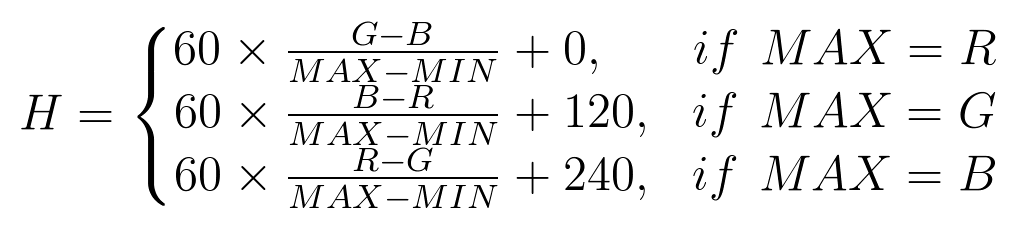
\includegraphics[width=0.5\hsize]{image201003/neuralnet05.png}
\end{center}
\end{figure}

$B%b%N%/%m2hA|$O?'Aj$r;}$?$J$$$?$a!"(BRGB$B$N$&$A@D$N@.J,$r8:$i$9$3$H(B
$B$G2+?'$$%U%#%k%?$r$+$1$^$7$?!#$3$&$9$k$3$H$G%b%N%/%m2hA|$N?'Aj$N(B
$BJ?6Q$O2+?'$H$J$j!"%+%i!<$H%b%N%/%m$rH=JL$9$k$?$a$NF~NOCM$H$7$F4|(B
$BBT$G$-$^$9!#(B

\if0
HSV$B$KJQ49!"(BH$B$NCM$r8+$k(B

$BGr$O(BHSV$B$K$J$$$N$G!"@D$r<e$/$7$F$_$k!#(B

$B2+?'$r8+$k!#(B

$B2+?'$@$1$N2hA|$N>l9g$O!&!&!&(B
\fi

\dancersection{weka$B$r;H$C$F$_$k(B}{$BA0ED9LJ?(B}
\subsection{$B35MW(B}
\subsection{$B%$%s%9%H!<%k(B}

Debian $B$G$O%Q%C%1!<%8$,MQ0U$5$l$F$$$^$9!#(B

\begin{commandline}
$ sudo apt-get install weka
\end{commandline}

\subsection{weka$B$N;H$$J}(B}

$B%3%^%s%I%i%$%s$G(B \texttt{weka} $B%3%^%s%I$r<B9T$7$^$9!#(B

\begin{commandline}
$ weka &
\end{commandline}

weka $B$N%&%#%s%I%&$,5/F0$7$^$9!#(B

\begin{figure}[H]
\begin{center}
\caption{Weka $B5/F0%a%K%e!<(B}
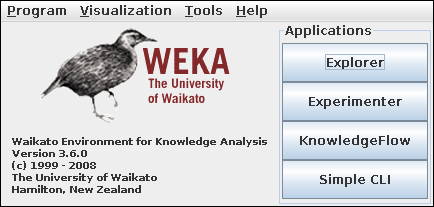
\includegraphics[width=0.5\hsize]{image201003/weka0.png}
\end{center}
\end{figure}

``Applications'' $B$N(B ``Explorer''$B$r<B9T$7$^$9!#(B

\begin{figure}[H]
\begin{center}
\caption{Weka Explorer}
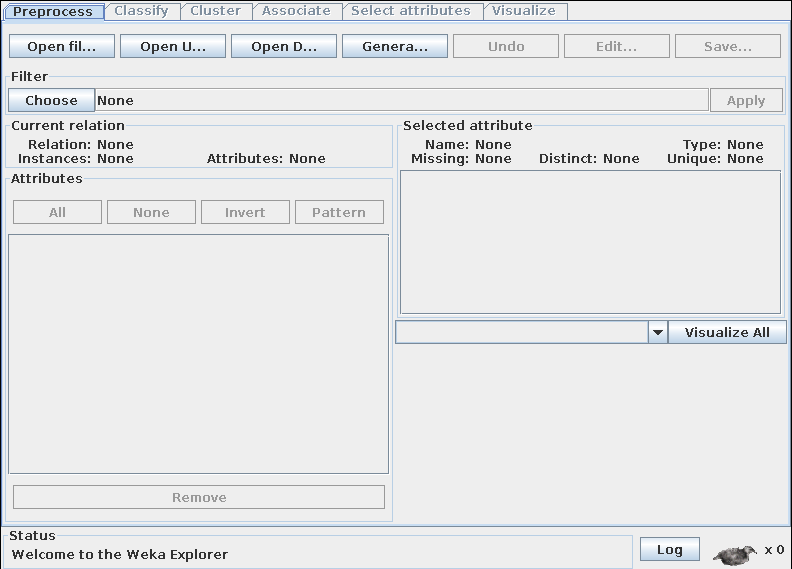
\includegraphics[width=1.0\hsize]{image201003/weka1.png}
\end{center}
\end{figure}

Weka Explorer $B$,5/F0$7$^$9!#(B

\subsubsection{ARFF$B%U%!%$%k$r%m!<%I$9$k(B}

Preprocess $B%?%V(B

Open File

/image200812/memberanalysis/attend.arff

\subsubsection{$B2D;k2=$7$F$_$k(B}

Visualize $B%?%V(B

$BE,Ev$K3+$/!#(B

\subsubsection{$BJ,N`$7$F$_$k(B}

Classify $B%?%V(B

Choose 
Multilayer Perceptron ($B%K%e!<%i%k%M%C%H%o!<%/$GJ,N`(B)

(Num)attendance $B$rL\E*4X?t(B

\subsection{$B;29MJ88%(B}
\begin{itemize}
 \item \url{www1.doshisha.ac.jp/~mjin/R/23.pdf}
 \item \url{http://web.sfc.keio.ac.jp/~soh/dm03/man_w_03.html}
\end{itemize}

\dancersection{man-db $B$r?<DI$$$7$?(B}{$BF|HfLn(B $B7<(B}

\subsection{$BF|K\8l$N(B man $B$,JQ(B}

$B$3$s$J46$8(B

\par
\includegraphics[width=100mm]{image201003/manls.eps}

\subsection{$B2r$O(Bgroff$B$K$"$j(B}

XXXX

$B?<DI$$$7$?7k2L$r:\$;$k(B

$B2r7h0F(B($B8=;~E@$G$NA[A|(B)$B$r7G:\!#(B

$B%5%9%Z%s%9$b$N!#(B

%-------------------------------------------------------------------------------
\dancersection{Debian $B$G(B libfftw $B$r;H$C$F$_$k(B}{$B>e@n=c0l(B}
%-------------------------------------------------------------------------------

\subsection{$B$O$8$a$K(B}

Debian$B$G(BFFT$B$r<h$j07$&(BC$B$N%"%W%j%1!<%7%g%s$r=q$$$F$_$?$$$H;W$&$3$H$O$"$j(B
$B$^$;$s$+(B?$B:#F|$O2;@<%G!<%?$rJ,@O$7$F$_$^$7$g$&!#(B

wav $B%U%!%$%k$rF~NO$H$7$F<u$1<h$j!"(BFFT$B$r<B9T$7$F$=$N7k2L$rI=<($9$k%"%W%j%1!<(B
$B%7%g%s$r:n@.$7$F$_$^$9!#(B

\subsection{$BF~NOCM$N=`Hw(B}

$BE,Ev$K(B wav $B%U%!%$%k$rMQ0U$7$^$7$g$&!#(B

$B:#2s$O<j85$G!"(Baeolus $B$r5/F0$7!"(B jack $B$G@\B3$5$;!"(Becasound $B$r(B jack $BF~NO$K(B
$BBP$7$FBT5!$5$;!"(Bqjackctl $B$G@\B3$5$;$F<}O?$7$^$7$?!#(B

\begin{commandline}
$ qjackctl &
$ aeolus &
$ vkeybd &
$ ecasound -i jack -o test.wav
ctrl-C $B$GCfCG(B
$ sweep test.wav # $BE,Ev$KJT=8(B

$ file ra-mono.wav 
ra-mono.wav: RIFF (little-endian) data, WAVE audio, Microsoft PCM, 16 bit, mono 44100 Hz
\end{commandline}
%$

\subsection{$B%$%s%9%H!<%k(B}

libfftw3 $B$r%$%s%9%H!<%k$7$^$9!#(B
$B$"$H!"2;@<%U%!%$%k$r%m!<%I$9$k$?$a$K(B sndfile1 $B$rMxMQ$7$^$9!#(B

\begin{commandline}
$ apt-get install libfftw3-dev libsndfile1-dev
\end{commandline}
%$

\subsection{sine $BGH$r:n@.$9$k(B}

$B$H$j$"$($:%F%9%HMQ$K(B 440Hz $B$NGH7A$r:n@.$7$^$9!#(B

\begin{commandline}
/*BINFMTC: -lsndfile -lm

  Create a sine wave at 44.1kHz for 1 second called sine.wav
 */
#include <stdlib.h>
#include <stdio.h>
#include <sndfile.h>
#include <math.h>

int create_sine(const char* filename, int size, double frequency)
{
  SF_INFO sfinfo = {
    .frames = size,
    .samplerate = 44100,
    .channels = 1,
    .format = SF_FORMAT_WAV | SF_FORMAT_PCM_16,
    .sections = 0,
    .seekable = 0
  };
  SNDFILE* s = sf_open(filename, SFM_WRITE, &sfinfo);
  double* data = malloc(sizeof(double) * size);
  int i;

  for (i=0; i < size; ++i)
    {
      data[i] = sin(frequency * 2.0 * M_PI * i / 44100.0);
    }

  sf_writef_double(s, data, size);
  sf_close(s);
  return 0;
}

int main()
{
  return create_sine("sine.wav", 44100, 440.0);
}
\end{commandline}
\subsection{FFTW$B$r;H$C$F(B wav $B%U%!%$%k$r=hM}$7$F$_$k(B}

sndfile $B$H(B fftw3 $B$r;H$C$F%U!<%j%(JQ49$7$F=PNO$r%@%s%W$7$F$_$^$7$g$&!#(B

\begin{commandline}
/*BINFMTC: -lsndfile -lfftw3 -lm
 */

#include <stdlib.h>
#include <stdio.h>
#include <sndfile.h>
#include <math.h>
#include <complex.h>
#include <fftw3.h>

/*
  process with FFTW
 */
void study_sound(double* data, int size)
{
  fftw_complex* spectrum;
  fftw_plan p;
  int i;

  spectrum = (fftw_complex*) fftw_malloc(sizeof(fftw_complex) * (size / 2 + 1));
  p = fftw_plan_dft_r2c_1d(size, data, spectrum, FFTW_ESTIMATE);

  /* process with FFTW */
  fftw_execute(p);

  /* dump output in CSV format */
  printf("i,abs,arg\n");
  for (i=0; i<(size/2+1); ++i) {
    printf("%i,%f,%f\n", i,
	   cabs(spectrum[i]),
	   carg(spectrum[i]) / 2.0 / M_PI * 360.0);
  }
  fftw_destroy_plan(p);
  fftw_free(spectrum);
}

/*
  Process wav file.

  @return 1 on failure, 0 on success.
*/
int process_wav_file(const char* filename, int size)
{
  SF_INFO sfinfo = {0, 0, 0, 0, 0, 0};
  SNDFILE* s = sf_open(filename, SFM_READ, &sfinfo);
  double* data = malloc(sizeof(double) * size);

  if (!s || !data)
    {
      fprintf(stderr,
	      "Something went wrong opening the file or allocating memory\n");
      return 1;
    }
  if (sfinfo.channels != 1)
    {
      fprintf(stderr,
	      "Please give me monaural audio data\n");
      return 1;
    }

  /* Read wav file into an array of double */
  sf_readf_double(s, data, size / sfinfo.channels);
  study_sound(data, size / sfinfo.channels);
  sf_close(s);
  return 0;
}

int main(int argc, char** argv)
{
  process_wav_file(argv[1], atoi(argv[2]));
  return 0;
}
\end{commandline}


$B<B9T$7$F$_$^$9!#(B

\begin{commandline}
$ ./sndfile-fftw.c sine.wav 44100 > sine.csv
$ ./sndfile-fftw.c ra-1sec.wav 44100 > ra.csv

\end{commandline}

\subsection{$B=PNO$r3NG'$7$F$_$k(B}

$B$H$j$"$($:4JC1$K%0%i%U$r:n@.$9$k$?$a$N%D!<%k$H$7$F(B R $B$r;H$C$F$_$^$7$g$&!#(B

\begin{commandline}
$ R

R version 2.7.1 (2008-06-23)
Copyright (C) 2008 The R Foundation for Statistical Computing
ISBN 3-900051-07-0

R$B$O%U%j!<%=%U%H%&%'%"$G$"$j!"!V40A4$KL5J]>Z!W$G$9!#(B 
 $B0lDj$N>r7o$K=>$($P!"<+M3$K$3$l$r:FG[I[$9$k$3$H$,$G$-$^$9!#(B 
$BG[I[>r7o$N>\:Y$K4X$7$F$O!"(B'license()'$B$"$k$$$O(B'licence()'$B$HF~NO$7$F$/$@$5$$!#(B 

R$B$OB?$/$N9W8%<T$K$h$k6&F1%W%m%8%'%/%H$G$9!#(B 
$B>\$7$/$O(B'contributors()'$B$HF~NO$7$F$/$@$5$$!#(B 
$B$^$?!"(BR$B$d(BR$B$N%Q%C%1!<%8$r=PHGJ*$G0zMQ$9$k:]$N7A<0$K$D$$$F$O(B 
'citation()'$B$HF~NO$7$F$/$@$5$$!#(B 
 
'demo()'$B$HF~NO$9$l$P%G%b$r$_$k$3$H$,$G$-$^$9!#(B 
'help()'$B$H$9$l$P%*%s%i%$%s%X%k%W$,=P$^$9!#(B 
'help.start()'$B$G(BHTML$B%V%i%&%6$K$h$k%X%k%W$,$_$i$l$^$9!#(B 
'q()'$B$HF~NO$9$l$P(BR$B$r=*N;$7$^$9!#(B 

> sine <- read.csv("sine.csv")
> ra <- read.csv("ra.csv")
> summary(sine)
       i              abs                 arg           
 Min.   :    0   Min.   :    0.000   Min.   :-179.9674  
 1st Qu.: 5512   1st Qu.:    0.000   1st Qu.:   0.0000  
 Median :11025   Median :    0.000   Median :   0.0000  
 Mean   :11025   Mean   :    1.000   Mean   :  -0.1395  
 3rd Qu.:16538   3rd Qu.:    0.000   3rd Qu.:   0.0000  
 Max.   :22050   Max.   :22049.319   Max.   : 180.0000  
> summary(ra)
       i              abs                 arg         
 Min.   :    0   Min.   :2.066e-03   Min.   :-179.93  
 1st Qu.: 5512   1st Qu.:1.467e-02   1st Qu.: -56.88  
 Median :11025   Median :1.907e-02   Median : -37.80  
 Mean   :11025   Mean   :3.944e-01   Mean   : -38.40  
 3rd Qu.:16538   3rd Qu.:3.620e-02   3rd Qu.: -17.82  
 Max.   :22050   Max.   :4.072e+02   Max.   : 180.00  

> plot(sine$i, sine$abs, xlim=c(400,500), ylim=c(0,22000), type="l")
> plot(ra$i, ra$abs, xlim=c(0,2000), ylim=c(0,100), type="l")
\end{commandline}

%\printindex

\cleartooddpage

\vspace*{15cm}
\hrule
\vspace{2mm}

\includegraphics[width=2cm]{image200502/openlogo-nd.eps}
\noindent \Large \bf Debian $BJY6/2q;qNA(B\\ \\
\noindent \normalfont \debmtgyear{}$BG/(B\debmtgmonth{}$B7n(B\debmtgdate{}$BF|(B \hspace{5mm}  $B=iHGBh(B1$B:~H/9T(B\\
\noindent \normalfont $BEl5~%(%j%"(B Debian $BJY6/2q(B $B!JJT=8!&0u:~!&H/9T!K(B\\
\hrule

\end{document}
